\documentclass{beamer}
\usepackage{amsmath}
\usepackage{amssymb}
\usepackage{nicefrac}
\usepackage{booktabs}
\usepackage{rotating}
\usepackage{multirow}
\usepackage{colortbl,color}
\usepackage{graphics}

\usepackage{colortbl,color}
\usetheme{material}
\useLightTheme
\usePrimaryOrange
\useAccentRed

\renewcommand{\theenumii}{\alph{\enumii}}
\defbeamertemplate{itemize subitem}{dash}{--}
\defbeamertemplate{itemize subsubitem}{dash}{--}
\setbeamertemplate{itemize item}[circle]
\setbeamertemplate{itemize subitem}[dash]
\setbeamertemplate{itemize subsubitem}[dash]
\setbeamertemplate{enumerate item}{\arabic{enumi}.}
\setbeamertemplate{enumerate subitem}{(\alph{enumii})}
\usefoottemplate{}

\setbeamertemplate{headline}{}
\usenavigationsymbolstemplate{}

\newcommand{\UNCOVER}[3]{\only<#2>{\color{white}{#1}}\only<#3>{#1}}
\newcommand{\UNCOVERR}[4]{\only<#2>{\color{white}{#1}}\only<#3>{\color{red}{#1}}\only<#4>{#1}}
\newcommand{\showOn}[3]{\only<#2>{\color<#2>{black} #1}\only<#3>{\color<#3>{white} #1}}
\newcommand{\SD}[1]{{\tiny $\left(#1\right)$}}
\newcommand{\SDm}[1]{{\tiny \left(#1\right)}}
\newcommand{\Prob}[1]{\mbox{Pr}\left\{#1\right\}}
\newcommand{\CProb}[2]{\mbox{Pr}\left\{#1\left|#2\right.\right\}}

\usepackage{array}
\newcolumntype{P}[1]{>{\centering\arraybackslash}p{#1}}


\newcommand{\indicator}[1]{\mathrm{1}\left\{{#1}\right\}}
\author{Alistair J. Wilson }
\date{Fall 2020\\ Information Transmission under the Shadow of the Future\\AEJ: Micro, 2020; DOI: 10.1257/mic.20170403}
\begin{document}

\title{Information Relationships}
\author{$\begin{array}{cc} \text{Alistair Wilson } & \text{Emanuel Vespa
}
\\ \text{\small Pittsburgh} & \text{\small UCSB }\end{array}$  }


\maketitle

\subsection{Intro}
\begin{frame}{Two main motivating questions}
\begin{card}
\textbf{Information:} Many information transmission problems have inefficient outcomes in static setting. Natural to ask:
\emph{Does repetition lead to more information revelation?}
\end{card}
\begin{card}
\textbf{Repeated Games:} As we move away from symmetric PD stage games, can this illuminate regularities in selection
\end{card}
\end{frame}

\begin{frame}
\begin{card}[Repetition and Information Transmission]
    \begin{itemize}
    \item Important topic in economics, accounting, finance and political science
    \item A large literature has examined one-shot strategic information transmission
        \begin{itemize}
            \item Theoretically
            \item Experimentally
        \end{itemize}
    \item Though the literature has focused on one-shot, many applied situations are repeated, ongoing relationships
    \item Does repetition help or hinder communication?
    \end{itemize}
\end{card}
\end{frame}

\begin{frame}
\begin{card}[Repeated Games]
    \begin{itemize}
        \item Information transmission is a naturally asymmetric relationship, one that embeds tensions over efficiency and distribution of payoffs
        \item Folk theorems, though theoretically elegant are essentially negative results
        \item Experiments can help reduce indeterminacy in our predictions by outlining behavioral regularities
    \end{itemize}
    \end{card}
\end{frame}

\begin{frame}
\begin{card}[Standard repeated PD game]
\begin{enumerate}
        \item Symmetric
        \item Unique efficient outcome
        \item Efficient play supported by:
            \begin{enumerate}
            \item ``Simple'' on-path play
            \item Harshest punishments are also ``simple''
            \end{enumerate}
    \end{enumerate}
\end{card}
\end{frame}

\begin{frame}
\begin{card}[Repeated Information game:]
    \begin{enumerate}
        \item Inherently asymmetric
        \item Potentially many efficient outcomes
        \item Efficient play represents a tradeoff
            \begin{itemize}
            \item Efficient outcomes with ``simple'' on-path play require complex punishments
            \item Simple supporting punishments require greater coordination on the path
            \end{itemize}
    \end{enumerate}
\end{card}
\end{frame}

% \begin{frame}{Question 2: Reduce Indeterminacy}
%     \begin{itemize}
%         \item Use experimental treatments that vary which efficient outcomes can
%         be supported with which punishments to understand selection
%         \item Find that ``simple'' punishments are focal
%         \item But ``simple'' punishments not sufficient without strong coordination
%         devices
%             \begin{itemize}
%                 \item Also need the efficient outcomes supported by Nash reversion to have
%                 ``simple'' on-path play
%             \end{itemize}
%     \end{itemize}
% \end{frame}

\begin{frame}
    \begin{card}[Game Set-up]
 Minimally simple:
        \begin{itemize}
            \item \textbf{Two players}: a sender and a receiver
            \item \textbf{Two states}: good or bad (left/right in exp.)
            \item \textbf{Two messages}: natural language framing to states
            \item \textbf{Three actions:} two risky options connected to states, and
            a safe option
        \end{itemize}
    \end{card}
\end{frame}

\begin{frame}
\begin{card}[Sender's Decision]
    \begin{center}
    \centering \includegraphics<1>[width=\textwidth]{./i/s2_table.eps}
    \end{center}
    \end{card}
\end{frame}

\begin{frame}
\begin{card}[Receiver's Decision]
\begin{center}
\centering \includegraphics<1>[width=\textwidth]{./i/s4_table.eps}
\end{center}
\end{card}
\end{frame}

\begin{frame}
\begin{card}[Payoffs]
	\begin{center}%
		\begin{tabular}{c|cc|c|c|}
		\multicolumn{1}{c}{} &  & \multicolumn{1}{c}{} & \multicolumn{2}{c}{State, $\theta$} \\ 
		\cline{4-5} 
		\multicolumn{1}{c}{} &  & \multicolumn{1}{c}{} & \multicolumn{1}{c}{Good} & \multicolumn{1}{c}{Bad} \\ 
		\cline{4-5} 
		Action, &  & Full & (1,1) & (1,0) \\ 
		\cline{4-5} 
		$a$ &  & Partial & ($\nicefrac{1}{3},\nicefrac{2}{3}$) & ($\nicefrac{1}{3},\nicefrac{2}{3}$) \\ 
		\cline{4-5} 
		 &  & None & (0,0) & (0,1) \\ 
		\cline{4-5} 
		\multicolumn{3}{c}{\emph{(Sender,Receiver)}} & \multicolumn{1}{c}{} & \multicolumn{1}{c}{} \\ 
		\end{tabular}
	\end{center}
\end{card}
\begin{card}
 \emph{Good} and \emph{Bad} are selected independently with equal probability
\end{card}
\end{frame}
\begin{frame}
\begin{card}[Payoffs]
	\begin{center}%
		\begin{tabular}{c|cc|c|c|}
		\multicolumn{1}{c}{} &  & \multicolumn{1}{c}{} & \multicolumn{2}{c}{State, $\theta$} \\ 
		\cline{4-5} 
		\multicolumn{1}{c}{} &  & \multicolumn{1}{c}{} & \multicolumn{1}{c}{Good} & \multicolumn{1}{c}{Bad} \\ 
		\cline{4-5} 
		Action, &  & Full & (1,1) & (1,0) \\ 
		\cline{4-5} 
		$a$ &  & Partial & ($\nicefrac{1}{3},\nicefrac{2}{3}$) & ($\nicefrac{1}{3},\nicefrac{2}{3}$) \\ 
		\cline{4-5} 
		 &  & None & (0,0) & (0,1) \\ 
		\cline{4-5} 
		\multicolumn{3}{c}{\emph{(Sender,Receiver)}} & \multicolumn{1}{c}{} & \multicolumn{1}{c}{} \\ 
		\end{tabular}
	\end{center}
\end{card}
\begin{card}
 Sender observes state, sends either ``Invest'' or ``Don't Invest''
	message
		\begin{itemize}
			\item Always prefers full investment
			\item Partial investment is the best option for an uninformed receiver
		\end{itemize}
\end{card}
\end{frame}

\begin{frame}
\begin{card}[Payoffs]
	\begin{center}%
		\begin{tabular}{c|cc|c|c|}
		\multicolumn{1}{c}{} &  & \multicolumn{1}{c}{} & \multicolumn{2}{c}{State, $\theta$} \\ 
		\cline{4-5} 
		\multicolumn{1}{c}{} &  & \multicolumn{1}{c}{} & \multicolumn{1}{c}{Good} & \multicolumn{1}{c}{Bad} \\ 
		\cline{4-5} 
		Action, &  & Full & (1,1) & (1,0) \\ 
		\cline{4-5} 
		$a$ &  & Partial & ($\nicefrac{1}{3},\nicefrac{2}{3}$) & ($\nicefrac{1}{3},\nicefrac{2}{3}$) \\ 
		\cline{4-5} 
		 &  & None & (0,0) & (0,1) \\ 
		\cline{4-5} 
		\multicolumn{3}{c}{\emph{(Sender,Receiver)}} & \multicolumn{1}{c}{} & \multicolumn{1}{c}{} \\ 
		\end{tabular}
	\end{center}
\end{card}
\begin{card}
\textbf{\emph{Good}} is the efficiency state (agreement
        over actions)
            \begin{itemize}
                \item Pareto ranking: $\text{Full}\succ_{\text{Good}}\text{Partial}\succ_{\text{Good}}\text{None}$
            \end{itemize}
\end{card}
\end{frame}
\begin{frame}
\begin{card}[Payoffs]
	\begin{center}%
		\begin{tabular}{c|cc|c|c|}
		\multicolumn{1}{c}{} &  & \multicolumn{1}{c}{} & \multicolumn{2}{c}{State, $\theta$} \\ 
		\cline{4-5} 
		\multicolumn{1}{c}{} &  & \multicolumn{1}{c}{} & \multicolumn{1}{c}{Good} & \multicolumn{1}{c}{Bad} \\ 
		\cline{4-5} 
		Action, &  & Full & (1,1) & (1,0) \\ 
		\cline{4-5} 
		$a$ &  & Partial & ($\nicefrac{1}{3},\nicefrac{2}{3}$) & ($\nicefrac{1}{3},\nicefrac{2}{3}$) \\ 
		\cline{4-5} 
		 &  & None & (0,0) & (0,1) \\ 
		\cline{4-5} 
		\multicolumn{3}{c}{\emph{(Sender,Receiver)}} & \multicolumn{1}{c}{} & \multicolumn{1}{c}{} \\ 
		\end{tabular}
	\end{center}
\end{card}
\begin{card}
\textbf{\emph{Bad}} is the distributional state (here constant sum)
            \begin{itemize}
                \item \textbf{Sender}: $\text{Full}\succ_{\text{Bad}}\text{Partial}\succ_{\text{Bad}}\text{None}$ 
                \item \textbf{Receiver}: $\text{None}\succ_{\text{Bad}}\text{Partial}\succ_{\text{Bad}}\text{Full}$ 
            \end{itemize}
\end{card}
\end{frame}


\begin{frame}
\begin{card}
    \begin{center}%
        \begin{tabular}{c|cc|c|c|}
        \multicolumn{1}{c}{} &  & \multicolumn{1}{c}{} & \multicolumn{2}{c}{State, $\theta$} \\ 
        \cline{4-5} 
        \multicolumn{1}{c}{} &  & \multicolumn{1}{c}{} & \multicolumn{1}{c}{Good} & \multicolumn{1}{c}{Bad} \\ 
        \cline{4-5} 
        Action, &  & Full & (1,1) & (1,0) \\ 
        \cline{4-5} 
        $a$ &  & Partial & ($\frac{1}{3},\frac{2}{3}$) & ($\frac{1}{3},\frac{2}{3}$) \\ 
        \cline{4-5} 
         &  & None & (0,0) & (0,1) \\ 
        \cline{4-5} 
        \multicolumn{3}{c}{\emph{(Sender,Receiver)}}
        \end{tabular}
    \end{center}
\end{card}
\begin{card}[Main Strategic Tensions]
    \begin{itemize}
        \item What to do as a sender when the state is \emph{Bad}?
        \item What to do as a receiver in reaction to \emph{Invest} message?
    \end{itemize}
    \end{card}
\end{frame}

% \begin{frame}
%     \begin{itemize}
%         \item ``Simple'' behaviors here:
%             \begin{itemize}
%                 \item \textbf{Sender:} \emph{Honesty} (Reveal State) vs. \emph{Deceive}
%                 (Always Invest)
%                 \item \textbf{Receiver:} \emph{Follow Message} vs. \emph{Safe Play} (Always
%                 Partial)
%             \end{itemize}
%     \end{itemize}
% \end{frame}

\begin{frame}
\begin{card}[Repetition]
  After every round there is:     
   \begin{itemize}
                \item a $\delta$ probability that the game continues for another round
                \item a $1-\delta$ probability that the supergame ends
            \end{itemize}
     Use $\delta=\tfrac{3}{4}$ across our sessions
\end{card}
    \begin{card}
     Precise history becomes common knowledge at end of each round
        \begin{itemize}
            \item Find out if sender lied
            \item Find out what receiver chose
        \end{itemize}
    \end{card}
\end{frame}

\begin{frame}
\begin{card}[Core Baseline Design]
   We implement this game under two set-ups    
   \begin{description}
                \item[Strangers] Matched to a new partner each round
                \item[Partners] Matched to same partner each round
  \end{description}
  Three sessions/46 subjects
\end{card}
\begin{card}[Assessment Metric]
   Focus on efficiency state: \emph{What fraction of the time is Full Investment selected in the Good state?}
\end{card}
\end{frame}

\begin{frame}
\begin{card}[Baseline Results: $\text{Prob}\left\{\text{Invest}|\text{Good}\right\}$]
    \begin{center}
    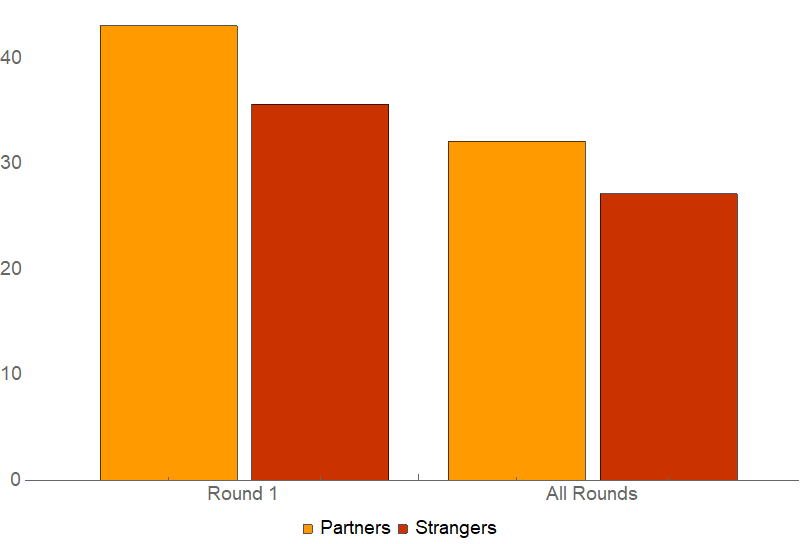
\includegraphics[width=0.95\textwidth]{./i/EffMain.png}
    \end{center}
\end{card}
\end{frame}

% \begin{frame}{Set of Payoffs and Individually Rational Payoffs}
% Focus on payoff space and characterize
% the set of individually rational payoffs, what is supportable with
% which punishments
% \end{frame}
\begin{frame}
\begin{card}[Summary]
   \begin{itemize}
    \item The \emph{Partners} game does do better than \emph{Strangers}
    \item But economically, as an effect it's not all that impressive
    \item Despite honest revelation being a Nash Equilibrium in Strangers, we do not see substantial honesty.
  \end{itemize}
\end{card}

\begin{card}
 \begin{center}
     Why?
 \end{center}
\end{card}
\end{frame}

% \begin{frame}{History-Dependent Strategies}
%     \begin{itemize}
%     \item With observation of the history in previous rounds
%         \begin{itemize}
%             \item Can use ``shadow of the future''
%             \item Focal conditional event: honesty in previous dealings 
%         \end{itemize}
%     \item Suppose the receiver wants to fully make use of the provided information
%     solely for their own gain
%         \begin{itemize}
%             \item This implies a required punishment
%         \end{itemize}
%     \end{itemize}
% \end{frame}



\begin{frame}
    \begin{card}[Explanations via Path \& Punishment]
    \begin{itemize}
        \item The simplest punishment cannot be used to support the receiver response of fully extracting
        \item Rather than using a bigger hard-to-wield stick, could also offer a better carrot
    \end{itemize}
    \end{card}
\end{frame}


% \begin{frame}
% \begin{card}
%     \begin{center}
%     \includegraphics<1>[height=0.75\textheight]{./i/feasibleIRpayoffsBase.eps}
%     \end{center}
% \end{card}
% \end{frame}

\begin{frame}
\begin{card}
    \begin{center}
    \includegraphics<1>[height=0.75\textheight]{./i/col_feasibleIRpayoffs5_1.eps}
    \end{center}
\end{card}
\end{frame}

\begin{frame}
\begin{card}
    \begin{center}
    \includegraphics<1>[height=0.75\textheight]{./i/col_feasibleIRpayoffs5_2.eps}
    \end{center}
\end{card}
\end{frame}

\begin{frame}{Information rents}
\begin{card}
 Goes back to Baron \& Besanko 1984; Laffont and Tirole 1988: 
        \begin{itemize}
        \item Honesty is not it's own reward
        \end{itemize}
 Threat of losing one's reputation for honest dealing can only
    induce good behavior if we punish deviators harshly, otherwise honesty needs to be rewarded with a `rent'
\end{card}
    \begin{card}
    With concavity in the payoffs this is a general feature of similar information transmission games for all $\delta\in(0,1)$
     \end{card}
\end{frame}

\begin{frame}
    \begin{card}[Question]
    Could failure to find efficiency improvements in Partners vs Strangers stem from strategic coordination failures?
    \end{card}
    \begin{card}[Diagnostic 1]
    Use the most powerful coordination device available to us in an experiment: \textbf{Preplay Chat}
    \begin{itemize}
        \item First 12 supergames same as Partners
        \item Supergames 13--20 the Sender/Receiver can chat before the supergame
    \end{itemize}
    \end{card}
\end{frame}

% \begin{frame}{Treatment games}
% \begin{itemize}
%     \item Our treatments vary which efficient outcome can be supported with
%     `simple' punishments
%     \item Two treatments in which:
% \begin{itemize}
%     \item Full Extraction can be supported with Nash Reversion
%     \item Info Rents equilibrium can be supported with Nash Reversion
% \end{itemize}
% \end{itemize}
% \end{frame}

% \begin{frame}{Nash=MinMax Treatment 1}
% \begin{center}

% \begin{tabular}{c|cc|c|c|}
% \multicolumn{1}{c}{} &  & \multicolumn{1}{c}{} & \multicolumn{2}{c}{State, $\theta$} \\ 
% \cline{4-5} 
% \multicolumn{1}{c}{} &  & \multicolumn{1}{c}{} & \multicolumn{1}{c}{Good} & \multicolumn{1}{c}{Bad} \\ 
% \cline{4-5} 
% Action, &  & Full & (1,1) & (1,0) \\ 
% \cline{4-5} 
% $a$ &  & Partial & ($\frac{1}{3},\frac{2}{3}$)$\rightarrow$($0,\frac{2}{3}$) & ($\frac{1}{3},\frac{2}{3}$)$\rightarrow$($0,\frac{2}{3}$) \\ 
% \cline{4-5} 
%  &  & None & (0,0) & (0,1) \\ 
% \cline{4-5} 
% \multicolumn{3}{c}{\emph{(Sender,Receiver)}} & \multicolumn{1}{c}{} & \multicolumn{1}{c}{} \\ 
% \end{tabular}
% \begin{itemize}
% \item Shift the sender's payoff under Nash down to the minmax
% \begin{itemize}
% \item Punishments now hurt more
% \end{itemize}
% \end{itemize}
% \end{center}
% \end{frame}

% \begin{frame}{Nash=MinMax Treatment 2}
% \begin{center}

% \begin{tabular}{c|cc|c|c|}
% \multicolumn{1}{c}{} &  & \multicolumn{1}{c}{} & \multicolumn{2}{c}{State, $\theta$} \\ 
% \cline{4-5} 
% \multicolumn{1}{c}{} &  & \multicolumn{1}{c}{} & \multicolumn{1}{c}{Good} & \multicolumn{1}{c}{Bad} \\ 
% \cline{4-5} 
% Action, &  & Full & (1,1) & (1,0) \\ 
% \cline{4-5} 
% $a$ &  & Partial & ($\frac{1}{3},\frac{2}{3}$) & ($\frac{1}{3},\frac{2}{3}$) \\ 
% \cline{4-5} 
%  &  & None & (0,0)$\rightarrow$($\frac{1}{3},0$) & (0,1)$\rightarrow$(\textrm{$\frac{1}{3},$}1) \\ 
% \cline{4-5} 
% \multicolumn{3}{c}{\emph{(Sender,Receiver)}} & \multicolumn{1}{c}{} & \multicolumn{1}{c}{} \\ 
% \end{tabular}
% \begin{itemize}
% \item Shift the sender's minmax up to the Nash payoff
% \begin{itemize}
% \item Better on-path payoff under full extraction; deviations less tempting
% \end{itemize}
% \end{itemize}
% \end{center}
% \end{frame}

% \begin{frame}{Baseline}
% \begin{center}
% \includegraphics<1>[height=0.8\textheight]{./i/feasibleIRpayoffsBase.eps}\includegraphics<2>[height=0.8\textheight]{./i/feasibleIRpayoffsMinMax.eps}\includegraphics<3>[height=0.8\textheight]{./i/feasibleIRpayoffsNash.eps}
% \end{center}

% \end{frame}\begin{frame}{Treatment 1 (T1)}
% \begin{center}
% \includegraphics<1>[height=0.8\textheight]{./i/feasibleIRpayoffsIR1.eps}\includegraphics<2>[height=0.8\textheight]{./i/feasibleIRpayoffsIR1Nash.eps}
% \end{center}

% \end{frame}
% \begin{frame}{Treatment 2 (T2)}
% 	\begin{center}
% \includegraphics<1>[height=0.8\textheight]{./i/feasibleIRpayoffsIR2.eps}\includegraphics<2>[height=0.8\textheight]{./i/feasibleIRpayoffsIR2Nash.eps}
% 	\end{center}
% \end{frame}

% \begin{frame}{Our Experiment}
% \begin{itemize}
% \item Nine treatment environments in total

% \begin{itemize}
% \item Three sessions per treatment
% \item 20 Supergames per session
% \item 16 participants per session
% \item Paid for three random supergames
% \end{itemize}
% \item First consider:

% \begin{enumerate}
% \item \textbf{Baseline}:
% \begin{itemize}
% \item Info Rents eq. supported with Babbling
% \item Full Extraction supported with MinMax
% \end{itemize}
% \item \textbf{Nash=MinMax} treatments: 
% \begin{itemize}
% \item Any IR efficient outcome supported with Babbling reversion
% \item Babbling payoffs in T1 = MinMax payoffs in Baseline
% \item Babbling payoffs in T2 = Babbling payoffs in Baseline
% \end{itemize}
% \end{enumerate}
% \end{itemize}
% \end{frame}

% \begin{frame} 
% \begin{center}

% \textbf{\textsc{\huge{}Top-Level Results}}{\huge\par}

% \end{center}\end{frame}

% \begin{frame}{Efficiency }
% \begin{center}
% Fraction of Good-state rounds with Full Investment minus Fraction
% of Good-state rounds with No Investment
% \par\end{center}

% \begin{center}
% 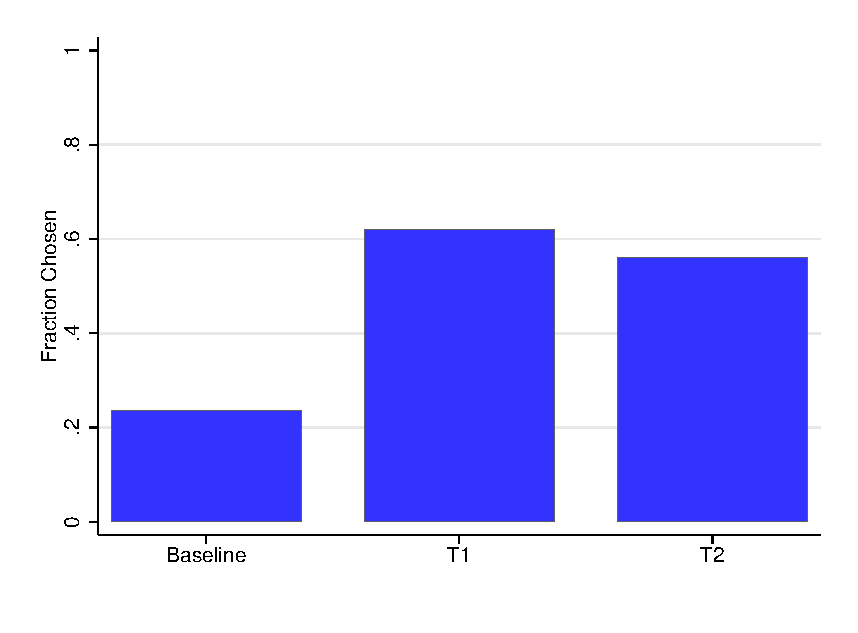
\includegraphics[scale=0.6]{./i/E1_L5A.eps}
% \par\end{center}
% \end{frame}

% \begin{frame}{Result \#1}

% Baseline Treatment 
% \begin{itemize}
% \item Modal behavior is the stage-game equilibrium.
% \item Almost all senders lie, claim good state
% \item Some evidence for history dependence, but economically small effect
% size
% \item Low Efficiency\bigskip{}
% \end{itemize}
% MinMax Treatments 
% \begin{itemize}
% \item Modal behavior is the efficient outcome with full extraction
% \item Senders fully reveal state
% \item Efficiency almost triples relative to baseline
% \end{itemize}
% \end{frame}
% \begin{frame}{On-Path Coordination Failures?}
% \begin{itemize}
% \item Get inefficient outcomes in our baseline; why did they not coordinate
% on the information-rents outcome that can be supported by the simple
% punishment
% \item \textbf{Hypothesis:} Failure in the baseline is due to a coordination
% failure over on-path play\bigskip{}
% \item \textbf{Chat Treatment}: 
% \begin{itemize}
% \item Use baseline parameterization
% \item Provide a powerful coordination device: pre-play communication
% \end{itemize}
% \end{itemize}
% \end{frame}

% \begin{frame}{Chat Treatments}
% \begin{itemize}
% 	\item Supergames 1 to 12, same as baseline
% 	\item Supergames 13 to 20 have pre-play communication
% 	\item 16 subjects, in perfect-stranger design for chat
% 	\item Chat happens before the supergame begins
% 	\begin{itemize}
% 		\item Purely coordinative
% 	\end{itemize}
% \end{itemize}
% \end{frame}

% \begin{frame}{Efficiency }
% \begin{center}
% Fraction of Good-state rounds with Full Investment minus Fraction
% of Good-state rounds with No Investment
% \par\end{center}

% \begin{center}
% 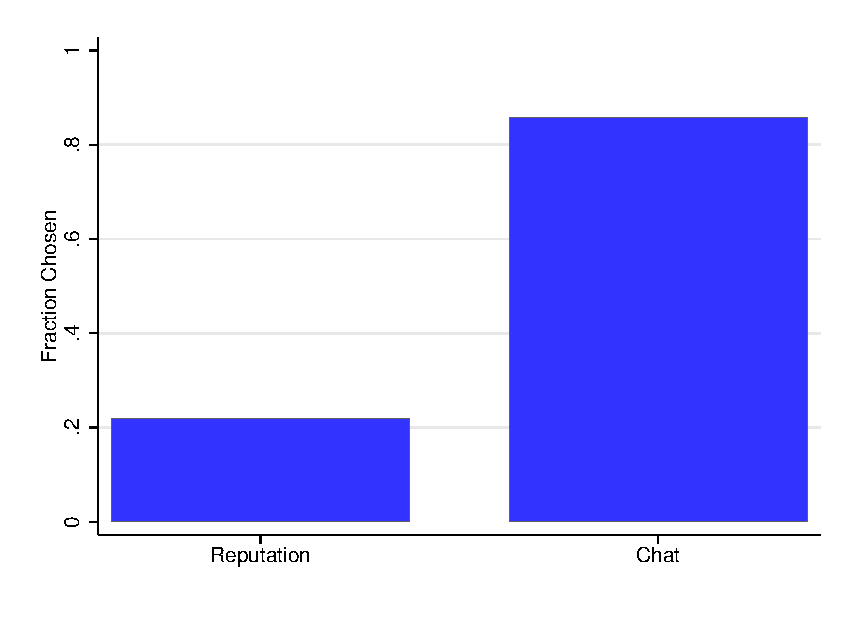
\includegraphics[scale=0.6]{./i/E1_ChatL5A.eps}
% \par\end{center}

% \end{frame}
\begin{frame}
\begin{card}[Chat Results: $\text{Prob}\left\{\text{Invest}|\text{Good}\right\}$]
    \begin{center}
    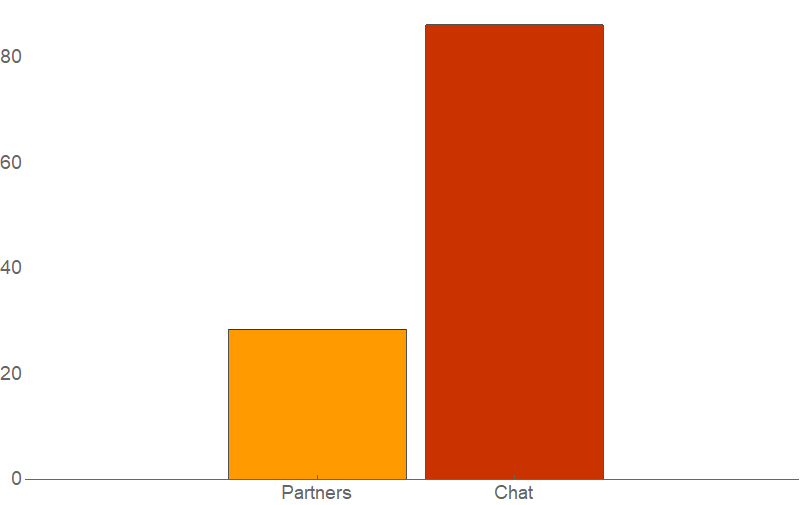
\includegraphics[width=0.95\textwidth]{./i/EffChat.png}
    \end{center}
\end{card}
\end{frame}

% \begin{frame}
%     \begin{card}[First Chat Supergames:]
%     \begin{quotation}
%     R(12): hello 
    
%     S(3): I'll always give you the correct recommendation if you choose
%     middle when I say right
%     \end{quotation}
%     \end{card}
% \end{frame}

\begin{frame}
    \begin{card}[First Chat Supergames:]
        \begin{quotation}
        R(4): no funny business/ :D 
        
        S(11): I'll tell you the actuall direction 
        
        S(11): i know 
        
        R(4): great 
        
        R(4): ill take middle if right 
        
        S(11): You're welcome
        \end{quotation}
    \end{card}
\end{frame}
\begin{frame}
    \begin{card}[First Chat Supergames:]
\begin{quotation}
       R(180): I'll trust you until you lie and then it's m,iddles the whole
way out. 

S(18): Hey want to work together on this? 

R(180): If you click right, I'll go middle so we both get something 

S(18): I will tell you all the honest computer decsions if you never
click right 

S(18): instead when i mark right click middle 

S(18): deal? 

R(180): no problem 

R(180): deal
\end{quotation}
    \end{card}
\end{frame}

\begin{frame}
    \begin{card}[Early Chat Supergame:]
\begin{quotation}
R(108): are you going to click honestly? 

S(198): I will give honest reccomendations if you choose middle when
i tell you RIGHT so we both benefit. That wil be my incentive to be
honst 

R(108): cool
\end{quotation}
    \end{card}
\end{frame}

\begin{frame}
    \begin{card}[Late Chat Supergame:]
\begin{quotation}
R(8): u right i middle 

S(9): when i say L, go L. when i say R, go middle 

R(8): Awesome same thought 
\end{quotation}
    \end{card}
\end{frame}

\begin{frame}
\begin{card}[Chat Evidence]
\begin{itemize}
    \item 78\% of chats articulate the information-rents outcome
    \item Clear that subjects understand this outcome as a possibility, but
    cannot coordinate on it without chat
    \item Deviations are punished with reversion to babbling
\end{itemize}
\end{card}
\end{frame}

\begin{frame}
\begin{card}[Coordination Result]
    \begin{itemize}
    	\item Chat drastically increases efficiency
    	\item Subjects clearly aware of information-rents path
    	\item Strategic uncertainty identified as cause of poor outcomes in Partners
    \end{itemize}
\end{card}
\begin{card}[Question]
    Can we weaken the coordination device?
\end{card}
\end{frame}

\begin{frame}
\begin{card}[Diagnostic 2]
    Add a version of Partners where we make the payment of a rent more explicit
    \begin{itemize}
        \item Add an option for the receiver to make a \$1 transfer ($\tfrac{1}{3}$ in normalized payoffs)
    \end{itemize}
\end{card}
\begin{card}
    This does not affect the individually rational payoffs of the game; just makes actions/intentions clearer
\end{card}
\end{frame}

\begin{frame}
\begin{card}[Explicit Receiver Transfer]
\begin{center}
\centering \includegraphics<1>[width=\textwidth]{./i/RecTip.png}
\end{center}
\end{card}
\end{frame}

\begin{frame}
\begin{card}[Results: $\text{Prob}\left\{\text{Invest}|\text{Good}\right\}$]
    \begin{center}
    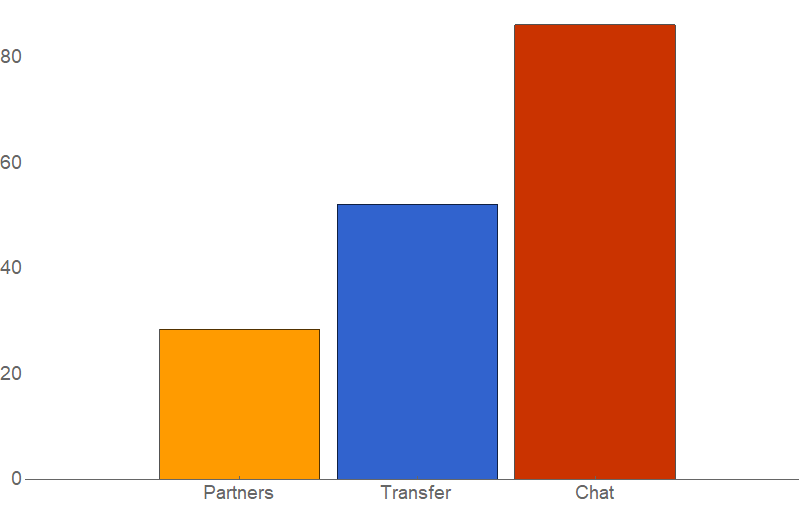
\includegraphics[width=0.95\textwidth]{./i/EffTip.png}
    \end{center}
\end{card}
\end{frame}

\begin{frame}
\begin{card}[Question]
    If we make Full Extraction supportable with Babbling reversion, do we get greater efficiency?
\end{card}
\begin{card}[Diagnostics 3 \& 4]
Manipulate sender's payoffs to achieve this
    \begin{itemize}
        \item Manipulation to the sender's payoff in the game achieve this 
    \end{itemize}
\end{card}
\end{frame}
\begin{frame}
\begin{card}[Baseline]
	\begin{center}%
		\begin{tabular}{c|cc|c|c|}
		\multicolumn{1}{c}{} &  & \multicolumn{1}{c}{} & \multicolumn{2}{c}{State, $\theta$} \\ 
		\cline{4-5} 
		\multicolumn{1}{c}{} &  & \multicolumn{1}{c}{} & \multicolumn{1}{c}{Good} & \multicolumn{1}{c}{Bad} \\ 
		\cline{4-5} 
		Action, &  & Full & (1,1) & (1,0) \\ 
		\cline{4-5} 
		$a$ &  & Partial & ($\nicefrac{1}{3},\nicefrac{2}{3}$) & ($\nicefrac{1}{3},\nicefrac{2}{3}$) \\ 
		\cline{4-5} 
		 &  & None & (0,0) & (0,1) \\ 
		\cline{4-5} 
		\multicolumn{3}{c}{\emph{(Sender,Receiver)}} & \multicolumn{1}{c}{} & \multicolumn{1}{c}{} \\ 
		\end{tabular}
	\end{center}
\end{card}
\end{frame}

\begin{frame}
\begin{card}[Manipulation 1]
	\begin{center}%
		\begin{tabular}{c|cc|c|c|}
		\multicolumn{1}{c}{} &  & \multicolumn{1}{c}{} & \multicolumn{2}{c}{State, $\theta$} \\ 
		\cline{4-5} 
		\multicolumn{1}{c}{} &  & \multicolumn{1}{c}{} & \multicolumn{1}{c}{Good} & \multicolumn{1}{c}{Bad} \\ 
		\cline{4-5} 
		Action, &  & Full & (1,1) & (1,0) \\ 
		\cline{4-5} 
		$a$ &  & Partial & ($\nicefrac{1}{3},\nicefrac{2}{3}$) & ($\nicefrac{1}{3},\nicefrac{2}{3}$) \\ 
		\cline{4-5} 
		 &  & None & ($\nicefrac{1}{3}$,0) & ($\nicefrac{1}{3}$,1) \\ 
		\cline{4-5} 
		\multicolumn{3}{c}{\emph{(Sender,Receiver)}} & \multicolumn{1}{c}{} & \multicolumn{1}{c}{} \\ 
		\end{tabular}
	\end{center}
\end{card}
\end{frame}

\begin{frame}
\begin{card}[Manipulation 2]
	\begin{center}%
		\begin{tabular}{c|cc|c|c|}
		\multicolumn{1}{c}{} &  & \multicolumn{1}{c}{} & \multicolumn{2}{c}{State, $\theta$} \\ 
		\cline{4-5} 
		\multicolumn{1}{c}{} &  & \multicolumn{1}{c}{} & \multicolumn{1}{c}{Good} & \multicolumn{1}{c}{Bad} \\ 
		\cline{4-5} 
		Action, &  & Full & (1,1) & (1,0) \\ 
		\cline{4-5} 
		$a$ &  & Partial & (0,$\nicefrac{2}{3}$) & (0,$\nicefrac{2}{3}$) \\ 
		\cline{4-5} 
		 &  & None & (0,0) & (0,1) \\ 
		\cline{4-5} 
		\multicolumn{3}{c}{\emph{(Sender,Receiver)}} & \multicolumn{1}{c}{} & \multicolumn{1}{c}{} \\ 
		\end{tabular}
	\end{center}
\end{card}
\end{frame}

\begin{frame}
\begin{card}[Results: $\text{Prob}\left\{\text{Invest}|\text{Good}\right\}$]
    \begin{center}
    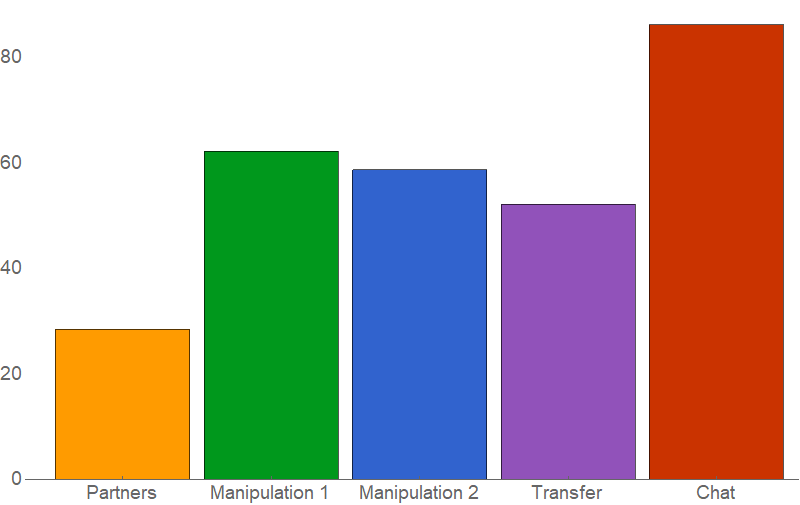
\includegraphics[width=0.95\textwidth]{./i/EffManip.png}
    \end{center}
\end{card}
\end{frame}

\begin{frame}
\begin{card}[Honesty is not it's own reward]
\begin{itemize}
    \item Implicit on-path information rents do not arise naturally
    \item Reducing strategic uncertainty improves outcomes, where information rents are focal
    \item Making the information rents explicit also improves outcomes
\end{itemize}
We only observe substantial revelation when honesty is paid for or
when dishonesty can be easily (and harshly) punished
\end{card}
\begin{card}
See paper for additional bells/whistles/significance-stars/mixture-model
estimates
\end{card}
\end{frame}

\begin{frame}
\begin{card}[Coordination]
Motivates more-restricted folk theorems where we modify available
punishments:
    \begin{itemize}
    \item Static-Nash folk theorem (Friedman 1971) as opposed to Minmax folk
    theorem (Fudenberg \& Maskin 1986)
    \end{itemize}
Outside of strongly symmetric environments, coordination problems are behaviorally very hard to overcome
    \begin{itemize}
    \item Without strong coordination devices, tacit cooperation/collusion harder to sustain
    \end{itemize}
\end{card}
\end{frame}


\end{document}
